%%%%%%%%%%%%%%%%%%%%%%%%%%%%%%%%%%%%%%
% LaTeX poster template
% Created by Nathaniel Johnston August 2009
% http://www.nathanieljohnston.com/2009/08/latex-poster-template/
%%%%%%%%%%%%%%%%%%%%%%%%%%%%%%%%%%%%%%

\documentclass[final]{beamer}
\usepackage[scale=1.24]{beamerposter}
\usepackage{graphicx}			% allows us to import images
\usepackage{bbm,amssymb,mathrsfs}
%\usepackage{natbib}
%\usepackage{graphicx,psfrag,dcolumn,amsmath,bm,color}
\usepackage{amssymb}
\usepackage{exscale}
\usepackage{textpos}
\usepackage[tight]{subcaption}
%-----------------------------------------------------------
% Define the column width and poster size
% To set effective sepwid, onecolwid and twocolwid values, first choose how many columns you want and how much separation you want between columns
% The separation I chose is 0.024 and I want 4 columns
% Then set onecolwid to be (1-(4+1)*0.024)/4 = 0.22
% Set twocolwid to be 2*onecolwid + sepwid = 0.464
%-----------------------------------------------------------

\newlength{\sepwid}
\newlength{\onecolwid}
\newlength{\twocolwid}
\newlength{\threecolwid}
\setlength{\paperwidth}{48in}
\setlength{\paperheight}{36in}
\setlength{\sepwid}{0.024\paperwidth}
\setlength{\onecolwid}{0.22\paperwidth}
\setlength{\twocolwid}{0.464\paperwidth}
\setlength{\threecolwid}{0.708\paperwidth}
\setlength{\topmargin}{-0.5in}
\usetheme{confposter}
\usepackage{exscale}

%-----------------------------------------------------------
% The next part fixes a problem with figure numbering. Thanks Nishan!
% When including a figure in your poster, be sure that the commands are typed in the following order:
% \begin{figure}
% \includegraphics[...]{...}
% \caption{...}
% \end{figure}
% That is, put the \caption after the \includegraphics
%-----------------------------------------------------------

\usecaptiontemplate{
\small
\structure{\insertcaptionname~\insertcaptionnumber:}
\insertcaption}

%-----------------------------------------------------------
% Define colours (see beamerthemeconfposter.sty to change these colour definitions)
%-----------------------------------------------------------

\setbeamercolor{block title}{fg=ngreen,bg=white}
\setbeamercolor{block body}{fg=black,bg=white}
\setbeamercolor{block alerted title}{fg=white,bg=dblue!70}
\setbeamercolor{block alerted body}{fg=black,bg=dblue!10}

%-----------------------------------------------------------
% Name and authors of poster/paper/research
%-----------------------------------------------------------

\title{
\includegraphics[scale=0.8]{RevisedPlainLogo.jpg}
Visualization and Causal Inference of the Mexican Drug War}
\author{Valeria Espinosa and Joseph Kelly \vskip0.5ex \small{vespinos@fas.harvard.edu, kelly2@fas.harvard.edu}}
\institute{Statistics Department, Harvard University}

% for some reason the textblock in the title was not letting me compile

% \title{\begin{textblock}{1}(0,0.32)
% 
\includegraphics[scale=0.8]{RevisedPlainLogo.jpg}
% \end{textblock}Visualization and Causal Inference of the Mexican Drug War}
% \author{Valeria Espinosa and Joseph Kelly \vskip0.5ex \small{vespinos@fas.harvard.edu, kelly2@fas.harvard.edu}}
% \institute{Statistics Department, Harvard University}%\\[\medskipamount]


%-----------------------------------------------------------
% Start the poster itself
%-----------------------------------------------------------

\begin{document}
\begin{frame}[t]
  \begin{columns}[t]												% the [t] option aligns the column's content at the top
    \begin{column}{\sepwid}\end{column}			% empty spacer column
    \begin{column}{\onecolwid}
 				\begin{block}{Problem Description}
	%	In Mexico, the presidency of Felipe Calder\'{o}n (2006-2012) has been characterized for the war against organized crime, raising many questions regarding security and violence. %We attempt to visualize and analyze homicide rates at the municipality level, and link this to information obtained about the association of drug cartels to municipalities.
		The main question of interest is: \textbf{do homicide rates increase significantly after a military intervention?}. Due to the observational nature we explored the feasibility of causal inference for the data obtained. 
%
		There are many challenges involved in answering this question. Here, we attempt to point them out and a first try at answering this question. As any good observational study, which mimics a randomized experiment, the \emph{design} and \emph{analysis} steps are clearly separated.
		
		
		      \end{block}
      \vskip2ex
      \begin{block}{Estimand}
 Following the Rubin Causal Model, let $Y_j(1)$ and $Y_j(0)$ denote the homicide rate of region $j$ one year after it received a military intervention, and what it would have been at that same point in time if it hadn't received the military intervention. The estimand of interest is the average causal effect of the military intervention for the regions that were intervened. That is $$\tau=\overline{Y}(1)-\overline{Y}(0)=\frac{\sum_j Y_j(1)-Y_j(0)}{J}.$$ % do we want to weigh these?
	For this case, we can think of the treated regions as the population of interest because in principle only regions like those are likely to receive a military intervention. We assume $Y_j(1)$ is observed for all treated units. Let $N_j$ denote the number of municipalities that correspond to region $j$, then 
	$$Y_j(1) = \sum_{i=1}^{N_j}w_{ij}Y_{ij}(1),$$
	where  $\textrm{Pop}_{j}= \sum_i^{N_j}\textrm{Pop}_{ij}$, and $$w_{ij}= \frac{\textrm{Pop}_{ij}}{\textrm{Pop}_{j}}.$$ 
	However, $Y_j(0)$ is missing for all $j$. Following the reasoning above, $$Y_j(0) = \sum_{i=1}^{N_j}w_{ij}Y_{ij}(0),$$ and all $Y_{ij}(0)$ are unobserved.
      \end{block}



      \vskip2ex

    \end{column}

    \begin{column}{\sepwid}\end{column}			% empty spacer column
    \begin{column}{\threecolwid}					  % create a three-column-wide column and then we will split it up later
      \begin{block}{Assumptions \& Challenges}
        \begin{itemize}
        \item \textbf{SUTVA} - stable unit treatment value assumption
          \begin{itemize}
          \item \textbf{No hidden values of treatments} A broad definition of what ``military intervention''- any mili means in this context helps us think of a two level treatment: receiving a military intervention (defined as ... see paper(that have resulted in deaths?)) or not receiving it.
          \item \textbf{No interference between units} The main idea is to group neighboring regions that have received military interventions in such a way that distances make the ``no interference'' assumption  more reasonable. For treated regions that are side to side were also assessed in terms of neighboring  geographic situation such as lack of highways connecting them %\url{http://mx.kalipedia.com/kalipediamedia/geografia/media/200805/11/geomexico/20080511klpgeogmx_4_Ges_SCO.png} or big mountains between them, or closeness to where the crops or smuggling routes are \url{http://utopiaguatemala.files.wordpress.com/2011/11/mexico_routes_in_466.gif} (can we find such data?).
            The last homicide rate that we have corresponds to 2010. That eliminated some of the interventions mentioned in the Nexos paper. 
            Following this reasoning 2213 municipalities were included in the initial control pool. Our 13 treated regions are:
		

            \begin{table}[ht]
              \begin{center}
		\begin{tabular}{llccccccc}
		  \hline
                  \textbf{unit}& \textbf{Region}& number of& Date of first & Within Region & SD Bin& SD Neyman &Effect- Gain&SD Neyman G\\
                  && municipalities& intervention& Effect&&& Score within&\\
		  \hline
                  1&\textbf{Tijuana} &   5 & 2008 &20.89 & 1.49 & 12.87&20.49 & 8.27 \\  
		2&		  \textbf{Nogales} &   5 & 2008 &36.97 & 5.37 & 33.51& 11.41 & 20.90 \\
		4&		  \textbf{Ju\'{a}rez} &  15 & 2009 & 195.11 & 3.84 & 88.33 & 192.99 & 79.88 \\   
		5&		  \textbf{P\'{a}nuco} &  14 & 2007 &  -0.90 & 0.92 & 0.39& 0.37 & 0.24 \\
		6&		  \textbf{Reynosa} &  24 & 2008 &  0.87 & 0.87 & 1.23  & -3.49 & 1.48 \\  
		8&		  \textbf{Guadalupe} &  20 & 2009 &  -5.06 & 0.59 & 0.89 & -4.27 & 0.58 \\  
		9&		  \textbf{Villa de Cos, Fresnillo} &  18 & 2008 &-1.35 & 1.24 & 0.44 & -2.87 & 0.34 \\  
		10&		\textbf{Te\'{u}l de Gonz\'{a}lez Ortega,} &10 & 2009&13.83 & 5.52 & 9.21& 7.32 & 4.99 \\ 
		11&		\textbf{Rinc\'{o}n de Romos} & 8 & 2008&-4.80 & 2.55 & 1.07& -4.10 & 1.05\\
		12&		\textbf{Sinaloa, Badiraguato, Pueblo Nuevo} &27 & 2007& 4.33 & 1.19 & 1.15 & -15.84 & 0.74 \\ 
		15&		\textbf{Celaya} &9 & 2009  &2.84 & 1.42 & 1.82& 6.74 & 1.37 \\ 
		16&		\textbf{Apatzing\'{a}n} &10 & 2007 &17.50 & 3.23 & 1.81 &-52.81 & 5.97 \\  
		18&		\textbf{Acapulco} &35 & 2008 & 12.45 & 1.47 & 1.86 & 1.19 & 0.77 \\ 
		&		 \textbf{Average}& 205& - &19.86& 0.78&  0.89&14.61& 0.79\\
			%   \textbf{7} &   5 & 2010* & \textbf{17} &6 & 2010* \\
			% \textbf{13} &11 & 2010* &  \textbf{14} &9 & 2010* \\ 
			% \textbf{3} &  12 & 2010
		\hline
              \end{tabular}
            \end{center}
          \end{table}
          update this table to have the number of municipalities that received the intervention AND the main names.
          Put the image of the intervention map next to it
        \end{itemize}
 
      \item \textbf{Unconfoundedness}: Unfortunately we didn't get experts to guide most of our decisions. However, we did get to interact with a couple of them and made our covariate choices based on the information received and our understanding of the relevant information. Our covariates include: location, political party before Calder\'{o}n, income 2006, education and medical information at 2005, percentage of indigenous language speakers, 2006 homicide rate at the municipality level, and GDP, Homicide Rate and Population at the state level.
      \item \textbf{Missing Data:} there were few treated units that had one covariate missing
				
      \end{itemize}	
      
      
  \end{block}
      \begin{columns}[t,totalwidth=\threecolwid]	% split up that three-column-wide column
        \begin{column}{\onecolwid}
			      \begin{block}{Estimation}
					Control municipalities are used to estimate each $Y_{ij}(0)$ to obtain an estimate $Y_j(0)$. We use propensity score matching to identify a set of control municipalities that look like the treated ones.
					Let $M_{ij}$ be the number of municipalities matched to the $i$th municipality in region $j$. Let $$\textrm{PopM}_{ij}=\sum_{k=1}^{M_{ij}}\textrm{PopM}_{ijk}$$ denote the total population of all $M_{ij}$ municipalities matched to the $i$th treated municipality in region $j$. Then 
					$$\hat{Y}_{ij}(0) =\sum_{k=1}^{M_{ij}}v_{ijk}Y_{ijk}(0),$$ where $v_{ijk}=\frac{\textrm{PopM}_{ijk}}{\textrm{PopM}_{ij}}.$
					Therefore,
					$$\hat{Y}_{j}(0) =\sum_{i=1}^{N_j}w_{ij}\hat{Y}_{ij}(0)=\sum_{i=1}^{N_j}w_{ij}\sum_{k=1}^{M_{ij}}v_{ijk}Y_{ijk}(0),$$
					and
					$$\hat{\tau}=\frac{\sum_j Y_j(1)}{J}-\frac{\sum_{j=1}^{J}\hat{Y}_j(0)}{J}.$$
			Note that this could be extended to using hierarchical models. We believe that using 
			An important 	
			      \end{block}
          \setbeamercolor{block title}{fg=red,bg=white}%frame color
          \setbeamercolor{block body}{fg=black,bg=white}%body color
          \begin{block}{Block Colours}
            For the standard blocks there are two colours; one for the title and one for the block body:\\
            \begin{semiverbatim}
              {\color{red}\\setbeamercolor}\{block title\}\newline \{fg=red,bg=white\}
            \end{semiverbatim}
            \begin{semiverbatim}
              {\color{red}\\setbeamercolor}\{block  body\}\newline \{fg=black,bg=white\}
            \end{semiverbatim}
            The \emph{fg} colour sets the text colour and \emph{bg} sets the background colour.
            For the normal blocks it makes no sense to use a background colour other than white. You \emph{can} change it, but it will look weird!
          \end{block}
        \end{column}
\begin{column}{\onecolwid}
\begin{block}{Homicide rate in 2007}
            \vspace{0.75in}
            \begin{center}
              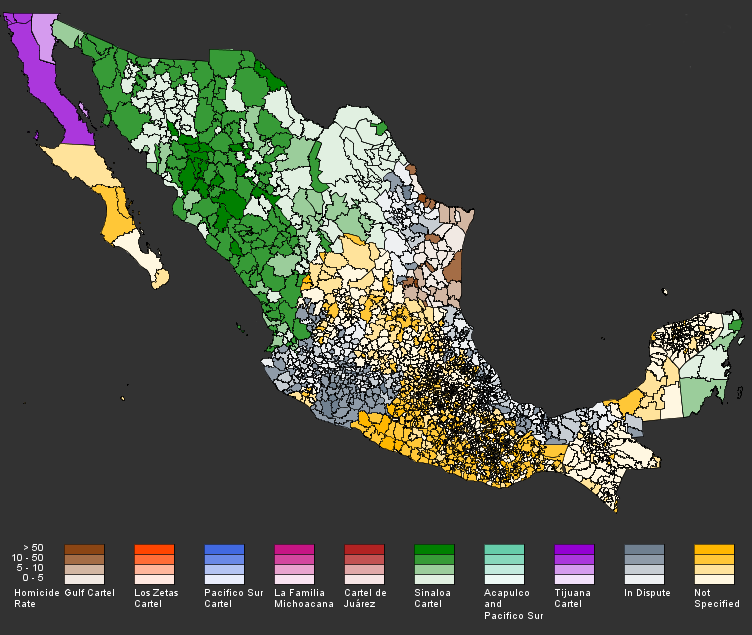
\includegraphics[width=7.2in]{2007.png}
            \end{center}
          \end{block}        
        \end{column}
        \begin{column}{\onecolwid}
          \begin{block}{Homicide rate in 2010}
            \vspace{0.75in}
            \begin{center}
              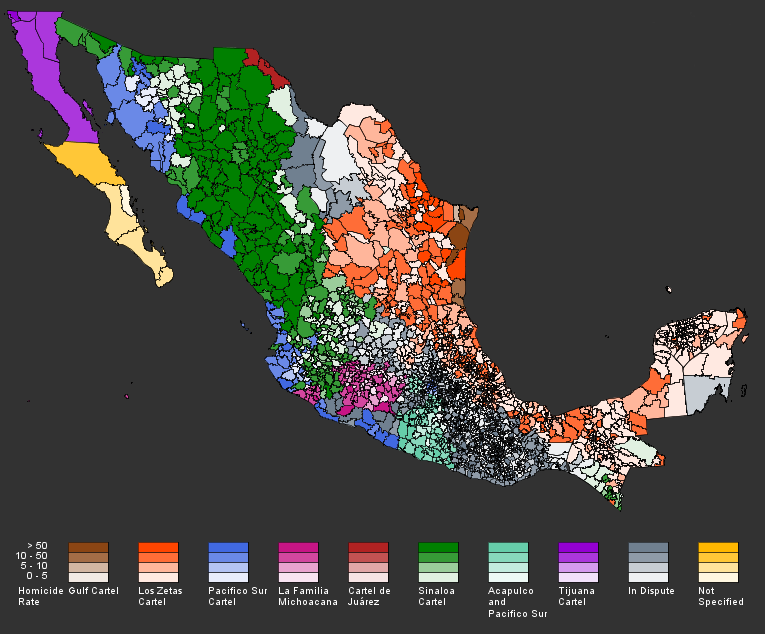
\includegraphics[width=7.2in]{2010.png}
            \end{center}
          \end{block}        
        %\end{column}
        %\begin{column}{\onecolwid}
          \begin{block}{Key References \& Data Source}
   
            \bibliographystyle{plain}
		        \small{\begin{thebibliography}{99}
				\bibitem{Abadie} Abadie  Synthetic Matching 
		        \bibitem{ImbensRubin} Imbens G. \& Rubin D.R., (2012)
				\bibitem{Rubin} Rubin D.R. ,\emph{Matched Sampling for Causal Effects},
				\bibitem{Valle} Diego Valle visualization
				\bibitem{CIDAC} CIDAC
				\bibitem{INEGI} INEGI
				\bibitem{SMaps} Stratfor Maps
		   \end{thebibliography}}

		      \end{block}
        \end{column}
      \end{columns}
      \vskip2.5ex
    \end{column}
  \begin{column}{\sepwid}\end{column}			% empty spacer column
 \end{columns}
\end{frame}
\end{document}
